\documentclass{article}

\usepackage{color}
\usepackage{graphicx}
\usepackage{amsmath}
\usepackage{bm}
\usepackage{enumerate}
\usepackage{booktabs}
\usepackage{cite}
\usepackage{geometry}
\usepackage{url}
\usepackage{float}
\usepackage{indentfirst}
\usepackage{ulem}
\usepackage{multirow}
\begin{document}

\vspace*{0.25cm}

\hrulefill

\thispagestyle{empty}

\begin{center}
\begin{large}
\sc{UM--SJTU Joint Institute \vspace{0.3em} \\ Introduction to Circuits \\(Ve215)}
\end{large}

\hrulefill

\vspace*{5cm}
\begin{Large}
\sc{{Laboratory Report}}
\end{Large}

\vspace{2em}

\begin{large}
\sc{{Lab 1
\vspace{0.5em}

DC Lab}}
\end{large}
\end{center}
\vfill

\begin{table}[h!]
\centering
\begin{tabular}{ll}
Name: Kang Jiaming \hspace*{2em}&
ID: 518021911220\hspace*{2em}\\

\\

Date:  2019.10.18

\end{tabular}
\end{table}

\hfill
\newpage


		\section{Introduction\label{intro}}
	\subsection{Objectives}
\noindent The goals for this lab are:
\begin{enumerate}
\item Learn how to use UT60A multimeter for measurements of voltage, current, and resistance. 
\item Learn to build circuits on a solderless prototype board. 
\item Verify the basic circuit laws –KCL, KVL, and Ohm’s laws from measurements of currents and voltages.
\item Measure the current-voltage characteristics of a 50$\Omega$ resistor. From the results of measurements, draw the conclusion on whether they obey Ohm’s law. 
\item Build an LED circuit on a protoboard and learn about non-ohmic circuit components, which do not obey Ohm’s law.  
\end{enumerate}
	\subsection{Apparatus and Theoretical Background}
\subsubsection{Multimeter}
A multimeter is able to work as a voltmeter to measure voltages, as an ammeter to measure currents, or as an ohmmeter to measure resistances.  Every multimeter has two terminals for the two cables that ensure electrical connections to the two nodes. The black cable should be connected to ground, the ground port is labeled COM on the multimeter. The red cable should be connected to HzV$\Omega$ port for voltage or resistance measurements, 10A MAX port for current measurements, or $\mu$AmA port for small current measurements.

\vspace{10pt}
\indent \textbf{Voltage Measurements} \\
\indent The voltmeter has its own internal resistance, which is usually very high. For an ideal voltmeter the input resistance is infinitely large. In real instruments the internal resistance usually exceeds 1M$\Omega$. When we measure VAB the voltmeter’s internal resistance is connected in parallel with all circuit elements between these two terminals. Note that you do not have to change anything in your circuit to measure voltage: just connect the multimeter to the nodes of interest.

\vspace{10pt}
\indent \textbf{Current Measurements} \\
\indent To measure the current that flows through a branch of your circuit we should make this current flow through the multimeter. Note that in order to measure the current we have to interrupt the circuit: the diagram below shows that instead of one node we work with two nodes A1 and A2.The circuits is broken at the point where we measure the current and the ammeter bridges the gap. The internal resistance of an ammeter is very low, say, 1$\Omega$ or less.
\begin{figure}[H]\centering
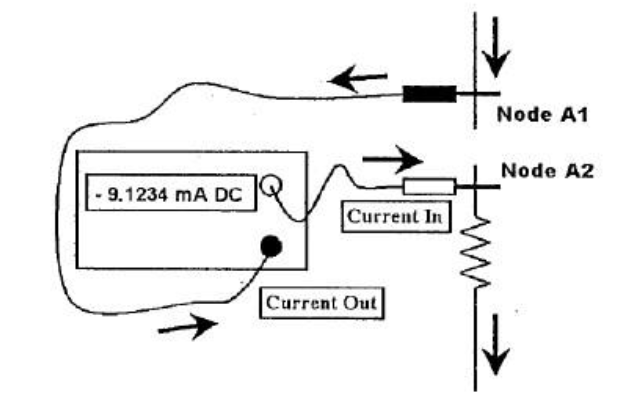
\includegraphics[scale=0.3]{current_measurements.png}
\caption{current measurements.}\label{figCurr}
\end{figure}

\vspace{10pt}
\indent \textbf{Resistance Measurements} \\
\indent To measure the resistance, we simply connect it to the two terminals of the multimeter, and read the resistance from the display. Remember: you must disconnect the resistor from your circuit before measuring the resistance! Otherwise, you will not obtain the correct reading of resistance. 

\subsubsection{DC source}

\vspace{10pt}
\indent \textbf{MOTECH LPS 305 Power Supply} \\
\begin{figure}[H]\centering
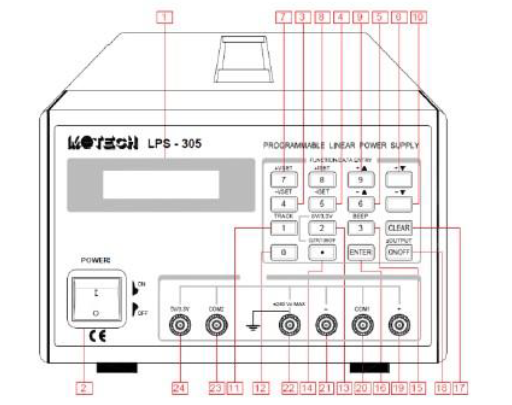
\includegraphics[scale=0.4]{supply1.png}
\caption{MOTECH LPS 305 Power Supply. (Retrieved from http://www.motech.com.tw/)}
\end{figure}
\begin{enumerate}
\item When you press the +Vset, or -Vset, the output selected (+output or –output) and the present setting for that function will be displayed. You can change setting using the numeric entry keys. Pressing the number keys will cause the present numeric setting to become blank and be replaced with the new numbers on the display. Pressing the ENTER key will enter the values displayed.
\item The selected output channel can be turned on and off from the front panel. The output on/off key toggles both the +output and –output on and off simultaneously.
\item Remember to turn off the output when no measurements are being undertaken.
\end{enumerate}

\vspace{10pt}
\indent \textbf{Agilent E3631A DC Power Supply} \\
\begin{figure}[H]\centering
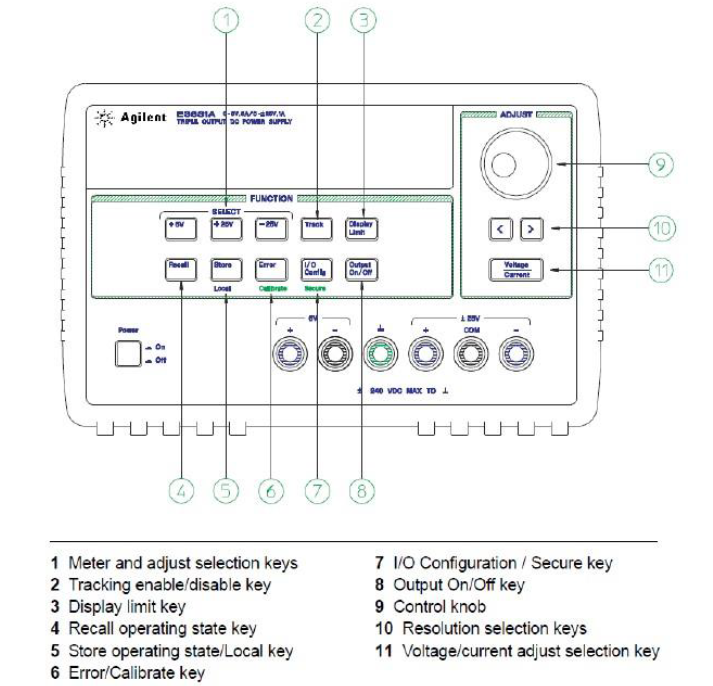
\includegraphics[scale=0.3]{supply2.png}
\caption{Agilent E3631A DC Power Supply. (Retrieved from http://cp.literature.agilent.com)}
\end{figure}
To set up the power supply for constant voltage (CV) operation, proceed as follows.
\begin{enumerate}
\item Connect a load to the desired output terminals with power-off. 
\item Press to turn on the power supply. The power supply will go into the power-on / reset state; all outputs are disabled (the OFF annunciator turns on); the display is selected for the +6V supply (the +6V annunciator turns on); and the knob is selected for voltage control. 
\item Adjust the knob for the desired output voltage. Set the knob for voltage control. The second digit of the voltmeter will be blinking. Adjust the knob to the desired output voltage. 
\end{enumerate}

\subsubsection{Protoboards}
In this lab and all the future labs, you will connect resistors, LEDs and other components to each other on a circuit board. Circuits boards are also called “protoboards”, because they are used for prototyping the circuits.  The main idea is to build the circuit without soldering every connection. A prototyping board used in the lab consists of several plastic blocks. These plastic blocks are mounted on a metal plate along with terminal (blind) posts. Each plastic block has many holes, into which you insert wires, plug in resistors, op amps, and other circuit components. Inside the plastic block, themetal clips snugly hold your wires, resistors, etc., and ensure electric connections between circuit components. Connections under the plastic are different for the wide and narrow blocks. Straight lines on the diagram above show the metal clips that connect holes under the plastic.
\begin{figure}[H]\centering
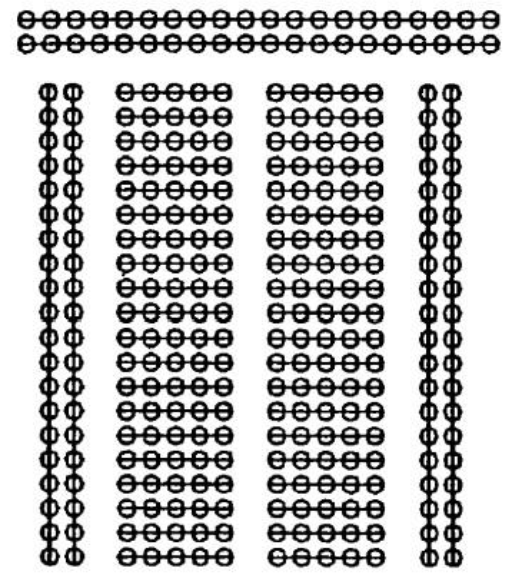
\includegraphics[scale=0.2]{board.png}
\caption{Protoboard.}\label{figProto}
\end{figure}

\subsubsection{Semiconductor diodes}
The simplest semiconductor device is a diode. Its circuit symbol looks like an arrow because the diode allows the current flow only in the direction of that arrow. If $V_A>V_B$ (which is called direct bias) the conductor will conduct. If $V_A<V_B$ (which is called reverse bias) the conductor will not conduct. Thus a diode is not an Ohmic resistor. 
\\
\begin{figure}[H]\centering
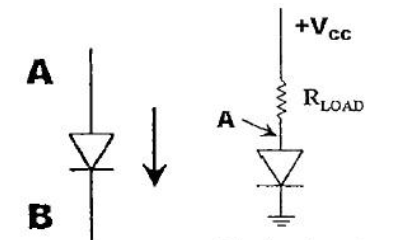
\includegraphics[scale=0.4]{diode.png}
\caption{Diode circuit.}
\end{figure}

Moreover, even under direct bias the resistance of a diode does not remain constant. At small values of the voltage difference $V_A-V_B$ the current through the diode is very small, because its resistance is large. The diode’s resistance abruptly changes as soon as the direct bias voltage across the diode reaches the threshold value, which is called the turn-on voltage and equals about 0.5 to 0.7V for many diodes. Above this voltage the current through the diode rapidly increases and becomes practically independent of the voltage. The diode resistance becomes so small that in real circuits the diodes have to be protected from high currents that may damage them. A load resistor (50$ \Omega $ in this lab) connected in series with the diode ensures the simplest protection.Light-emitting diodes emit light (visible or infrared) when the direct current becomes large enough. The LED, which you will use in this lab, has the turn-on voltage of about 1.6V.

		\section{Measurements}
	\subsection{Voltage, Current and Resistance Measurement}
	\begin{enumerate}
	\item Use the multimeter to measure the resistance R1 labeled 100$\,\Omega$ directly and record the result.
	\item Connect the resistance R1 = 100$\,\Omega$ with the power supply and set the voltage 3V.
	\item Use the multimeter to measure the Voltage (m) across the resistor.
	\item Use the multimeter to measure the Current (m) through the resistor.
	\end{enumerate}
	
	\subsection{Voltage Division and Current Division}
	\begin{enumerate}
	\item Before measurement, measure the actual resistances of the two resistors you are using in this section.
	\item Connect the R1 = 100$\,\Omega$ and R2 = 50$\,\Omega$ in series and in parallel, respectively.
	\item Use the multimeter to measure the voltage across the R1, R2 and the power supply.
	\item Use the multimeter to measure the current through R1, R2 and the power supply.
	\end{enumerate}
	
	\subsection{Ohm's Law}
	\begin{enumerate}
	\item  Measure the resistance of R = 50$\,\Omega$ and record the result.
	\item Connect the R with the power supply.
	\item Set the voltage outputs and record the corresponding currents.
	\item Sketch the voltage-current characteristic curve of the resistor.
	\end{enumerate}
	
	\subsection{Non-ohmic LED}
	\begin{enumerate}
	\item Connect the resistor R = 50$\,\Omega$ and the LED in series with the power supply.
	\item Change the voltage output and record the corresponding current.
	\end{enumerate}
	
		\section{Results and Discussion}
	\subsection{Voltage, Current and Resistance}
\begin{table}[H]\centering
\begin{tabular}{cccc}
\toprule
Resistance [$\Omega$] & \multicolumn{3}{l}{99.3}\\
\midrule
Voltage(m) [V] & 2.977 & Voltage(s) [V] & 3.000\\
Current(m) [A] & 0.030 & Current(s) [A] & 0.029\\
\bottomrule
\end{tabular}
\caption{Measurement of voltage, current, and Resistance.}\label{TableVAR}
\end{table}


The relative errors of the measurement of resistance is
$$u_R = \frac{100-99..3}{100}\times 100\% = 0.7\%.$$

	\subsection{Voltage Division and Current Division}
\begin{table}[H]\centering
\begin{tabular}{ccccc}
\toprule
& Resistance R1 [$\Omega$] & 99.3 & Resistance R2 [$\Omega$] & 46.4\\
\midrule
& \multicolumn{2}{c}{Voltage Division} & \multicolumn{2}{c}{Current Division}\\
& Current [A] & Voltage [V] & Current [A] & Voltage [V]\\
\midrule
Total & 0.020 & 2.990 & 0.093 & 2.984\\
R1 & 0.020 & 2.037 & 0.030 & 2.984\\
R2 & 0.020 & 0.951 & 0.064 & 2.984\\
\bottomrule
\end{tabular}
\caption{Voltage division and current division.}\label{TableDivision}
\end{table}

When the two resistors are in series, the current through the elements are the same and we can calculate the total voltage by
$$V_{\text{total}} = V_{\text{R1}}+V_{\text{R2}} 2.988 [\text{V}].$$
The relative error of total voltage is
$$u_V = \frac{2.988-2.990}{2.990}\times 100\% = 0.06\%.$$

When the two resistors are in parallel, the voltage between two nodes are the same and we can calculate the total current by 
$$I_{\text{total}} = I_{\text{R1}}+I_{\text{R2}} = 0.094 [\text{V}].$$
The relative error of total current is
$$u_I = \frac{0.094-0.093}{0.093}\times 100\% = 1.08\%.$$

It can be concluded that the division of voltage and current correspond with the basic laws of circuit that discussed in the lecture.


	\subsection{Ohm's Law}
\begin{table}[H]\centering
\begin{tabular}{cc}
\toprule
Resistance [$\Omega$] & 46.6\\
\midrule
Voltage [V] & Current [A]\\
\midrule
0.5 & 0.010\\
1.0 & 0.020\\
1.5 & 0.031\\
2.0 & 0.042\\
3.0 & 0.064\\
4.0 & 0.087\\
5.0 & 0.110\\
\bottomrule
\end{tabular}
\caption{Ohm's law.}\label{TableOhm}
\end{table}

\begin{figure}[H]\centering
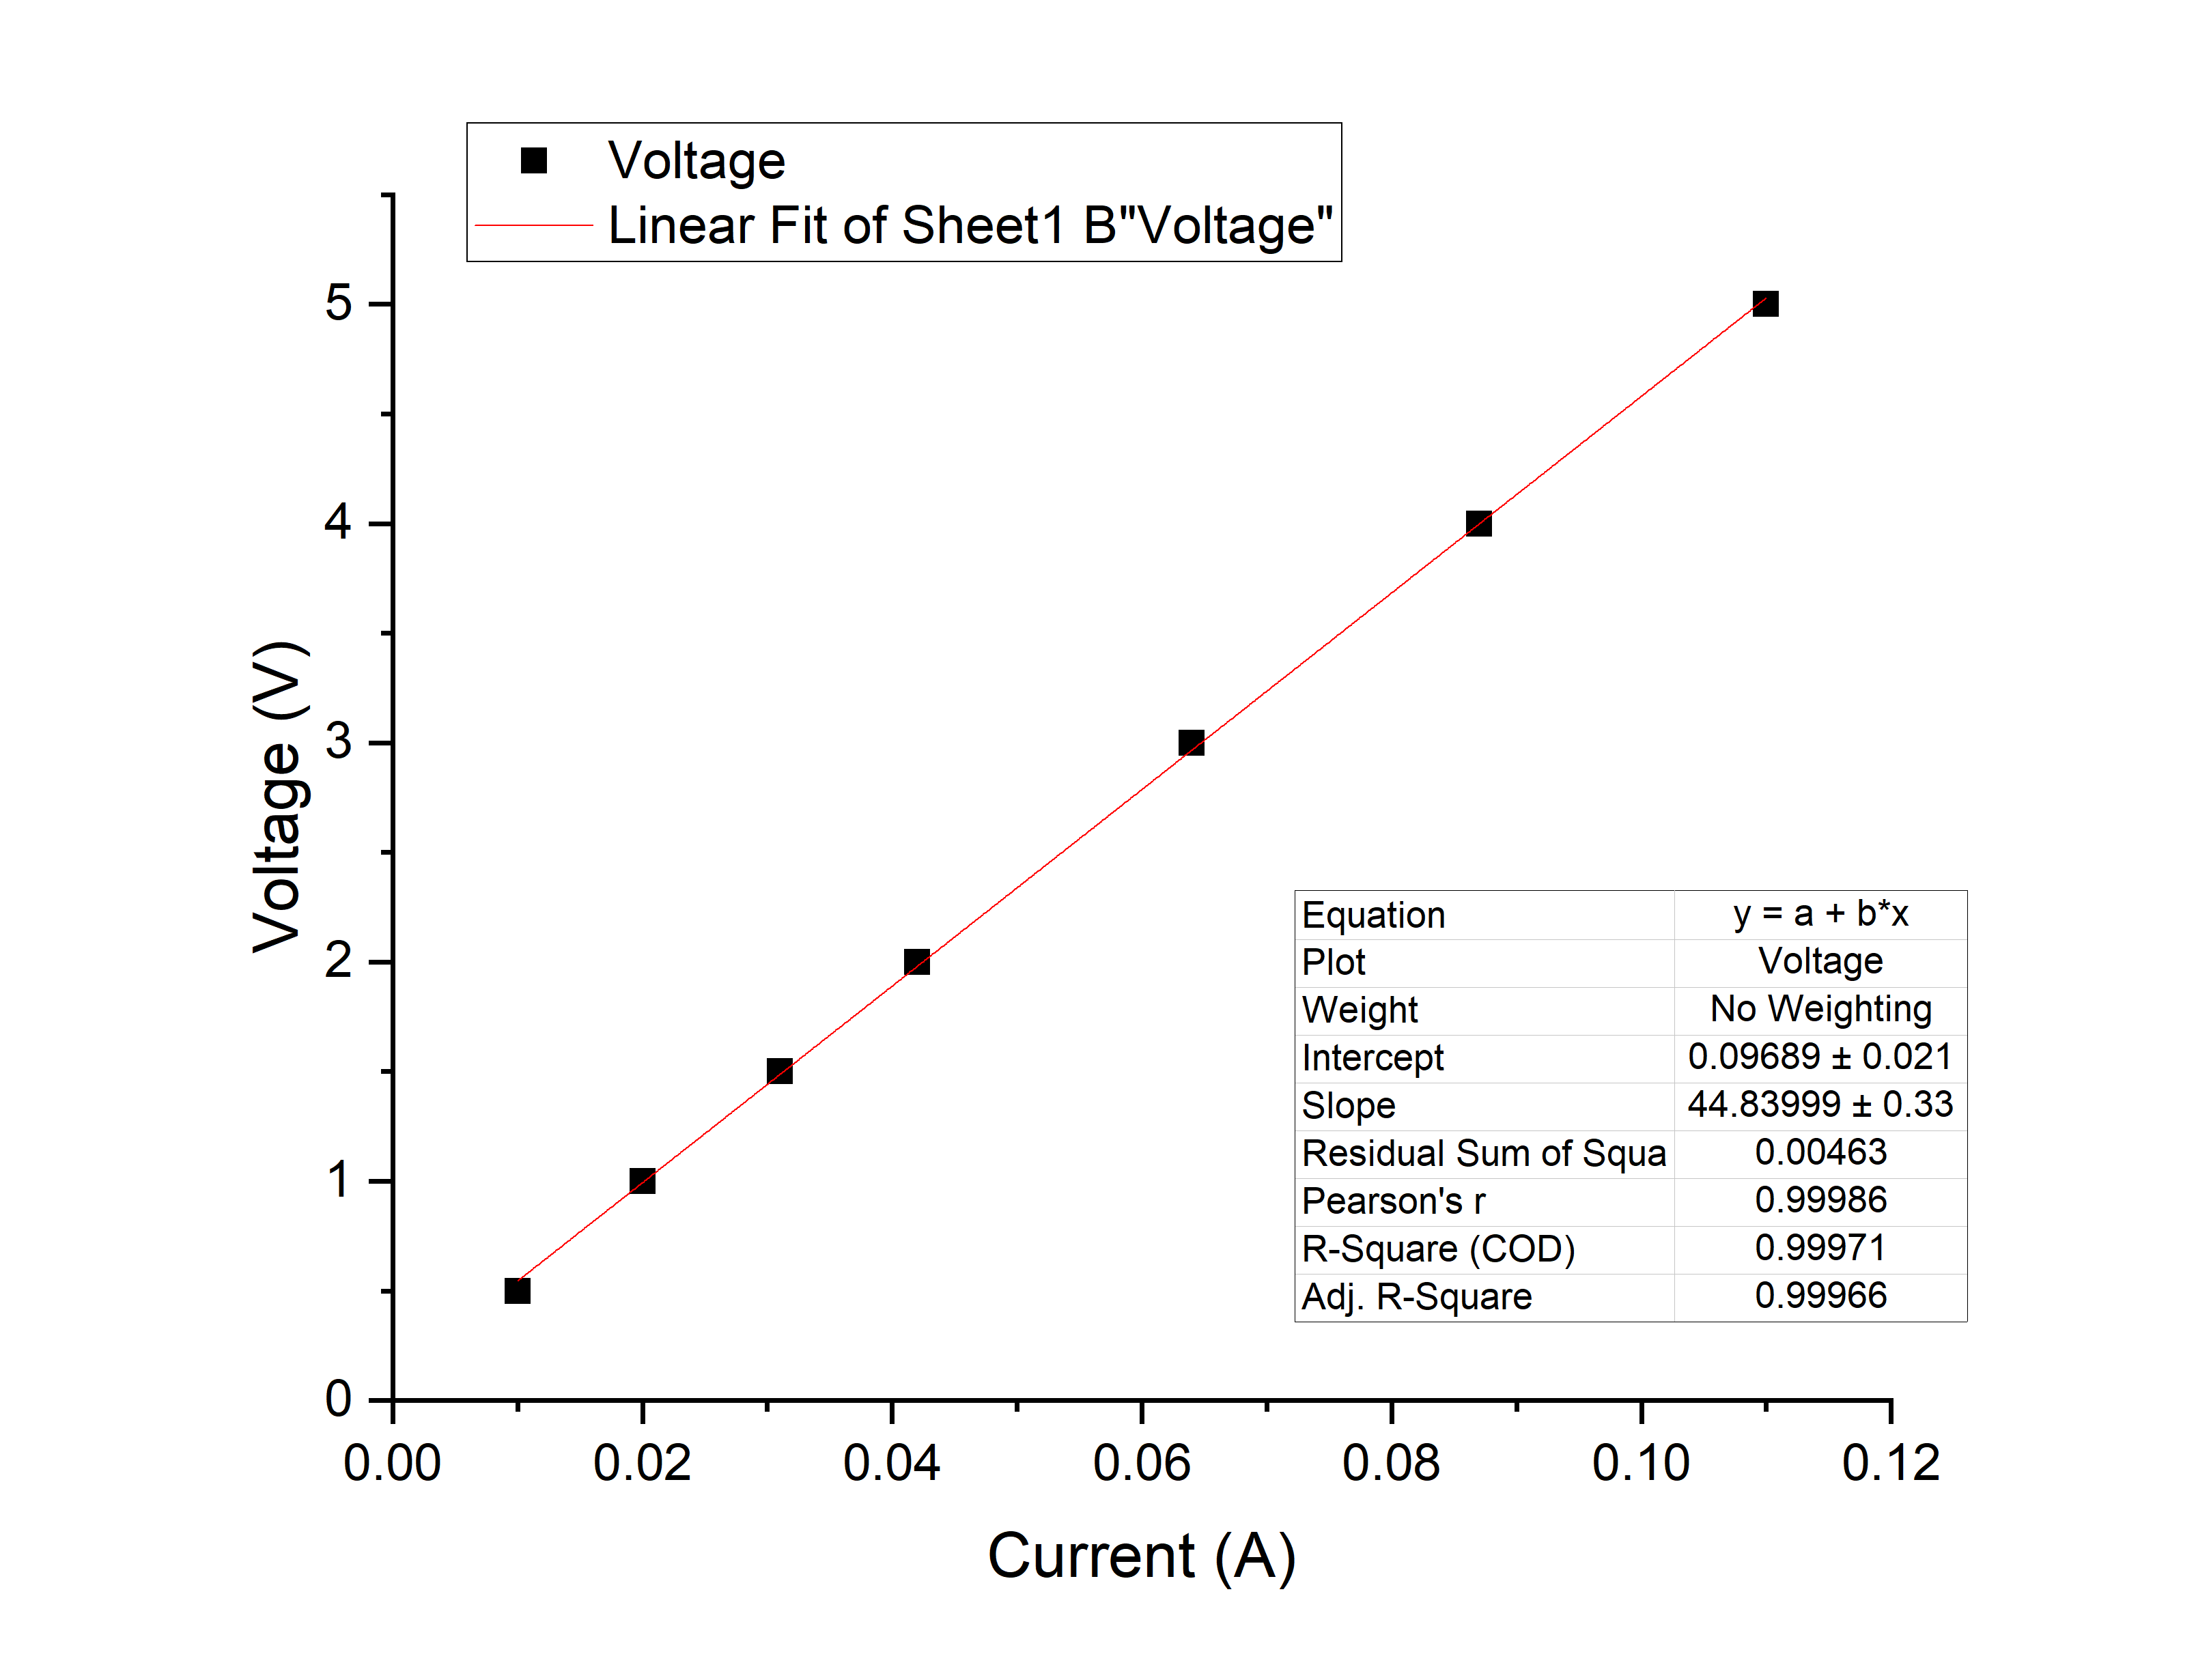
\includegraphics[scale=0.4]{Ohm.png}
\caption{Linear fit of voltage and current relation.}\label{FigOhm}
\end{figure}

Applying linear fit to the data using OriginLab, as shown in Figure \ref{FigOhm}, the slope of the fitting is the resistance, which is 44.8 $\Omega$.

The relative error is
$$u_R = \frac{46.6-44.8}{46.6}\times 100\% = 3.86\%.$$


	\subsection{Non-ohmic LED}
\begin{table}[H]\centering
\begin{tabular}{cc}
\toprule
Voltage [V] & Current [A]\\
\midrule
0.5 & 0.000\\
1.5 & 0.000\\
1.9 & 0.002\\
2.1 & 0.003\\
2.4 & 0.009\\
2.7 & 0.015\\
\bottomrule
\end{tabular}
\caption{Semiconductor diodes.}\label{TableDiode}
\end{table}

\begin{figure}[H]\centering
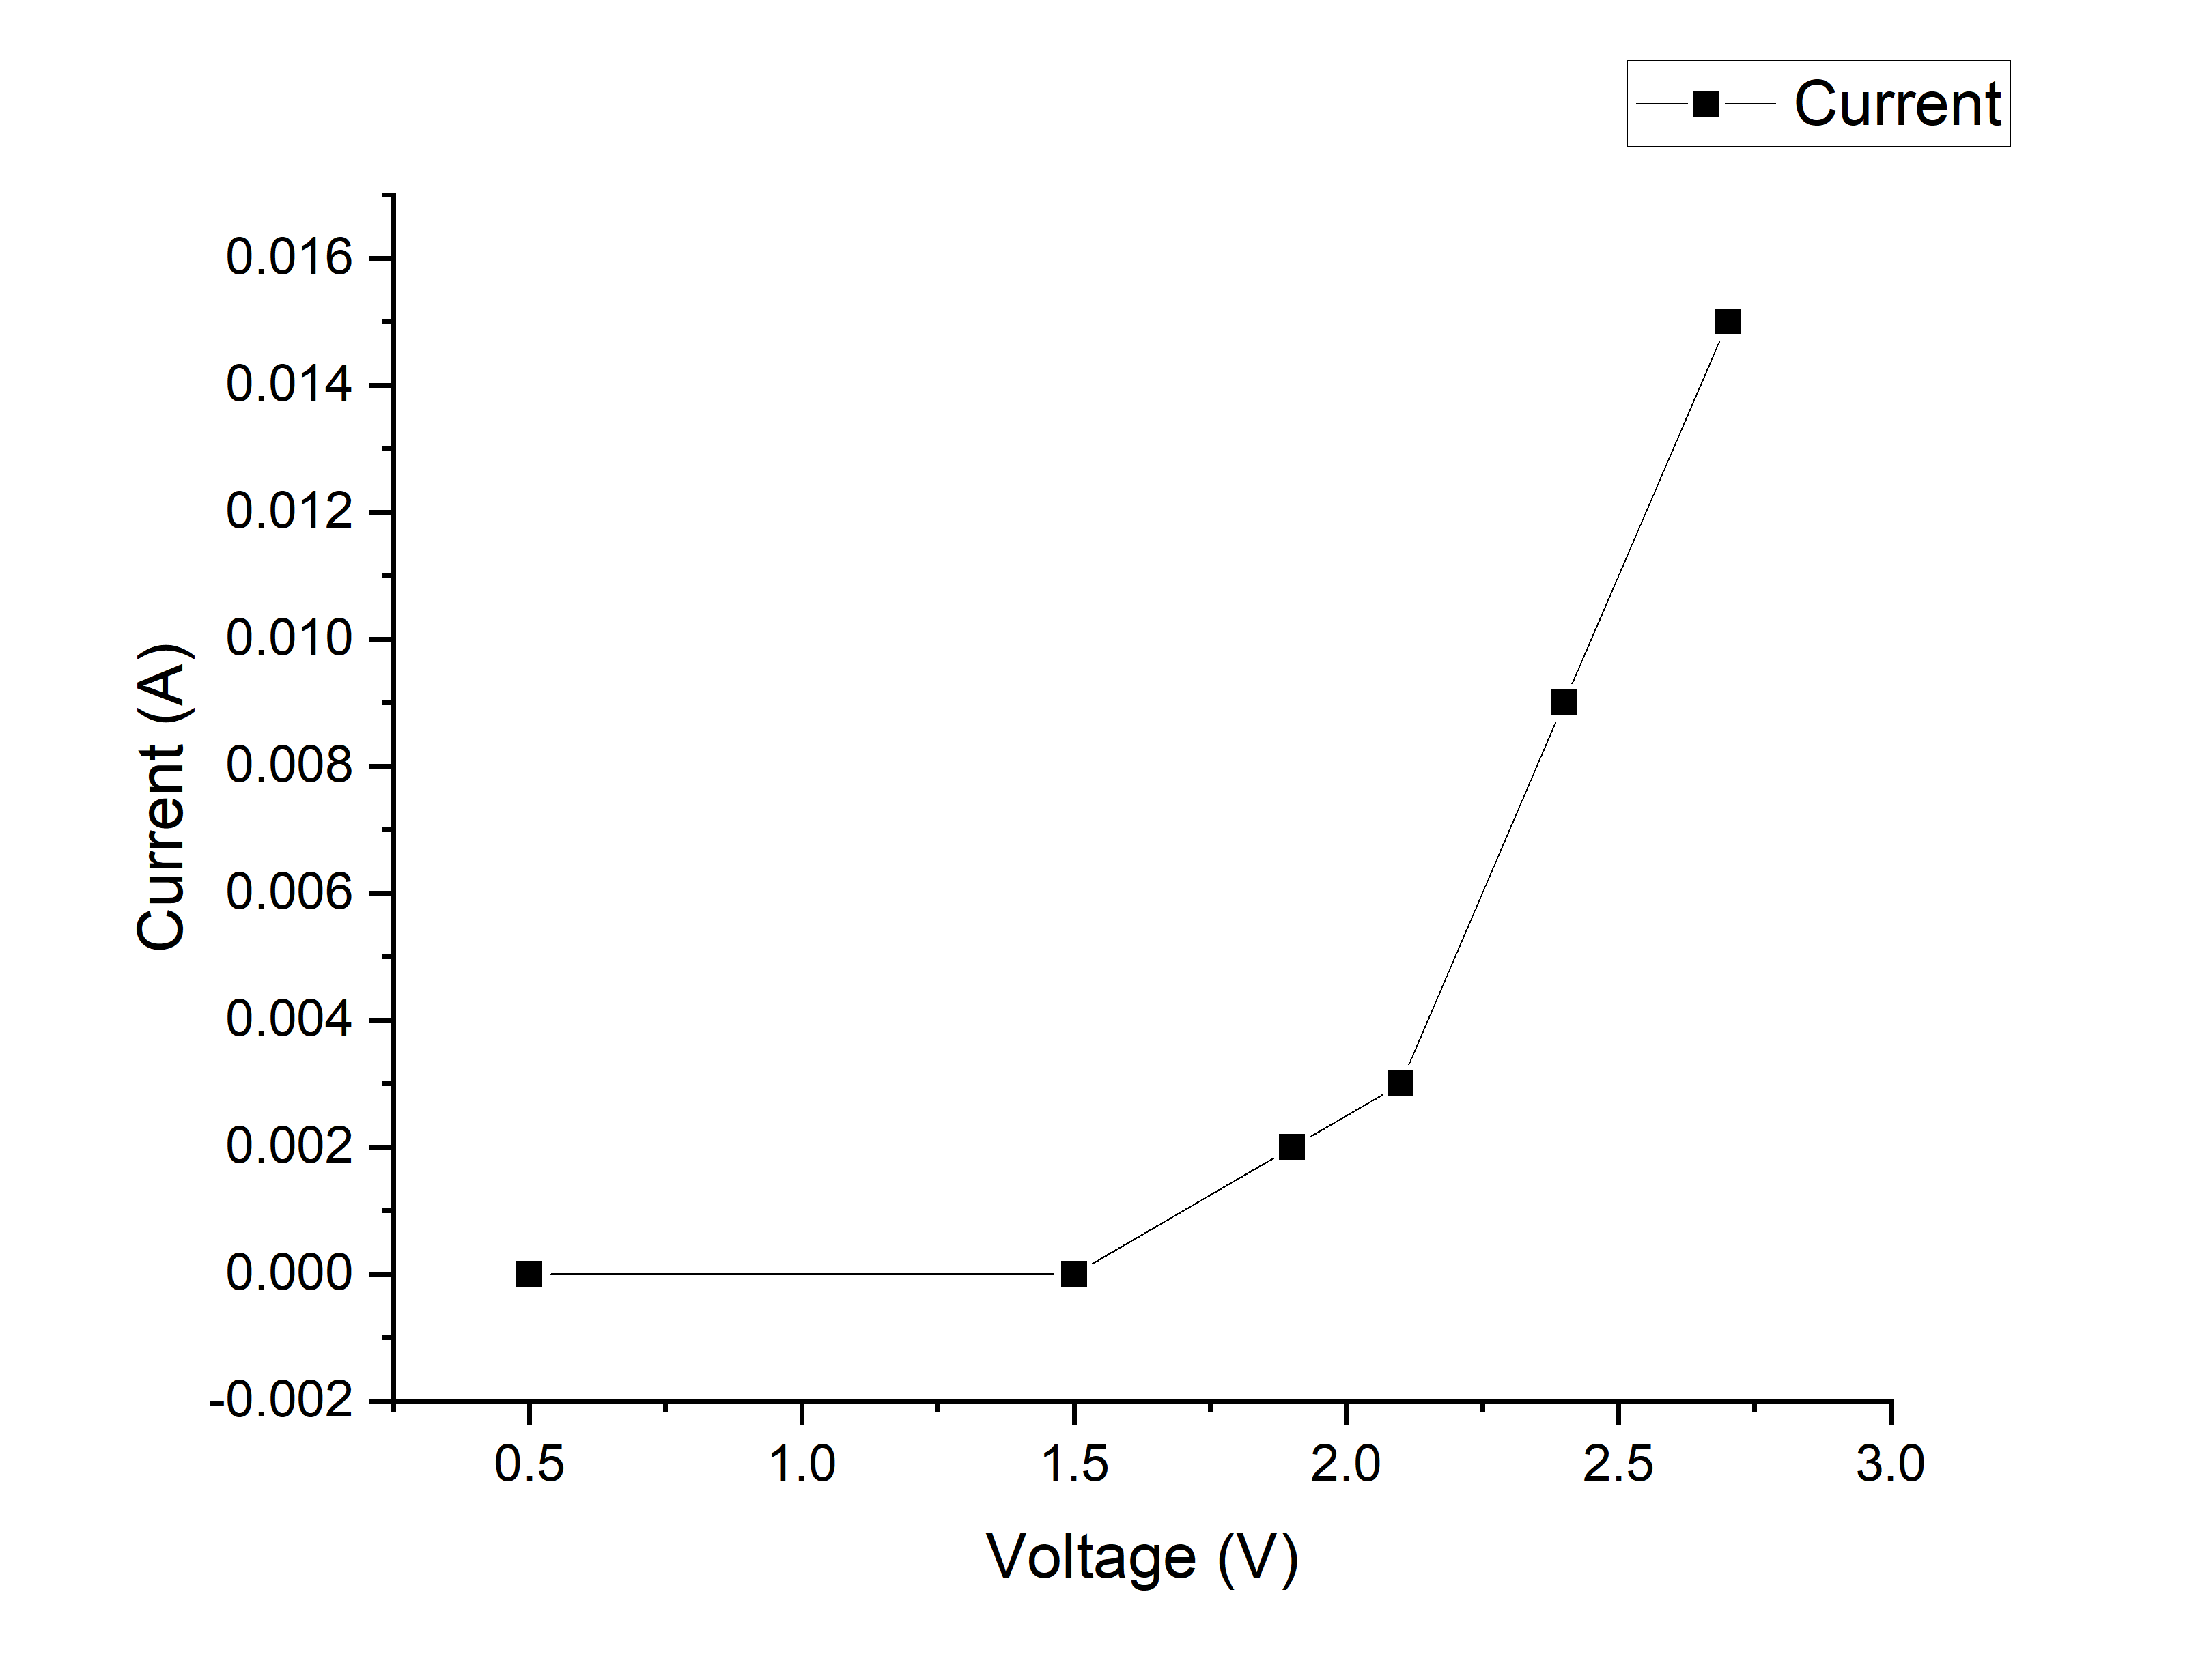
\includegraphics[scale=0.3]{Diode_measured.png}
\caption{Voltage-current relation of the diode.}\label{FigDiode}
\end{figure}

Figure \ref{FigDiode} shows the voltage-current relationship of diode. It can be seen that when the voltage applied on the diode is small, the current through it is very small. When the voltage applied on the diode reaches the turn-on value, the current through it increases rapidly. The turn-on voltage for the diode used in the experiment is about 1.6-1.8V, which agrees with the manual to an acceptable degree.



		\section{Conclusions}
In lab 1, we use the multimeter to measure the voltage, current and resistance and based on that, we verify the division of voltage and current and the Ohm's laws. We also try out constructing circuits on the prototype board.

The result of the experiment is desirable within an acceptable range of error. Some reasons may account for the errors. First, when connecting the circuit, we have to use our own hands because the protoboard does not work. Our body is connected in the circuit, which may lead to error of measurement. Besides, the resolution of the multimeter may also lead to error.

Despite such error, the result we obtain agrees with the expectation and basic laws of circuits. The graph we obtained is reasonable and informative. This experiment is relatively successful.


\section{References}
\noindent [1] VE215 Lab Manual Lab1:DC Lab Manual

\section{Appendix}
Attached find the data sheet.

\end{document}
